\documentclass{article}
\usepackage[UTF8]{ctex}
\usepackage{pythonhighlight}
\usepackage{markdown}
\usepackage{listings}
\lstset{
    basicstyle          =   \tt,          % 基本代码风格
    identifierstyle=\color{brown!80!black},
    keywordstyle        =   \color{purple}\bfseries,          % 关键字风格
    commentstyle        =   \rmfamily\itshape,  % 注释的风格,斜体
    stringstyle         =   \ttfamily,  % 字符串风格
    flexiblecolumns,                % 别问为什么,加上这个
    numbers             =   left,   % 行号的位置在左边
    showspaces          =   false,  % 是否显示空格,显示了有点乱,所以不现实了
    numberstyle         =   \zihao{-5}\ttfamily,    % 行号的样式,小五号,tt等宽字体
    showstringspaces    =   false,
    captionpos          =   t,      % 这段代码的名字所呈现的位置,t指的是top上面
    frame               =   lrtb,   % 显示边框
    backgroundcolor=\color[RGB]{245,245,244},
}


% Language setting
% Replace `english' with e.g. `spanish' to change the document language
\usepackage[english]{babel}
\usepackage{float}
% Set page size and margins
% Replace `letterpaper' with `a4paper' for UK/EU standard size
\usepackage[letterpaper,top=2cm,bottom=2cm,left=3cm,right=3cm,marginparwidth=1.75cm]{geometry}

% Useful packages
\usepackage{amsmath}
\usepackage{graphicx}
\usepackage[colorlinks=true, allcolors=blue]{hyperref}

\title{数逻实验报告Lab6}
\author{雷远航}

\begin{document}

\maketitle

\begin{abstract}
    实验项目:七段数码管
\end{abstract}

\section{操作方法与实验步骤}

\subsection{原理图设计实现显示译码模块MyMC14495}
\subsubsection{绘制原理图}
\subsubsection*{根据真值表绘制出七位译码器}
    \begin{figure}[H]
	\centering
	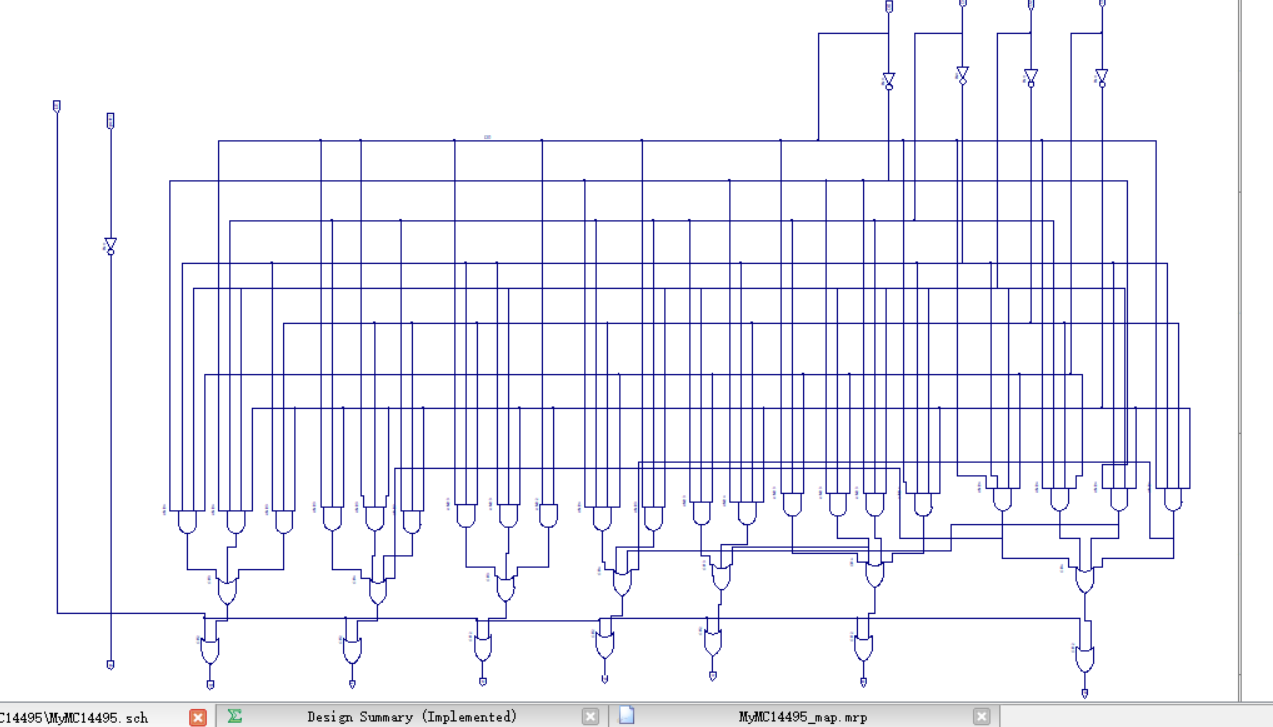
\includegraphics[width=0.9\textwidth]{1.png}
	\caption{\label{Lab6}原理图}
	\end{figure}

\subsubsection{对生成的原理图进行检验}
    \begin{figure}[H]
	\centering
	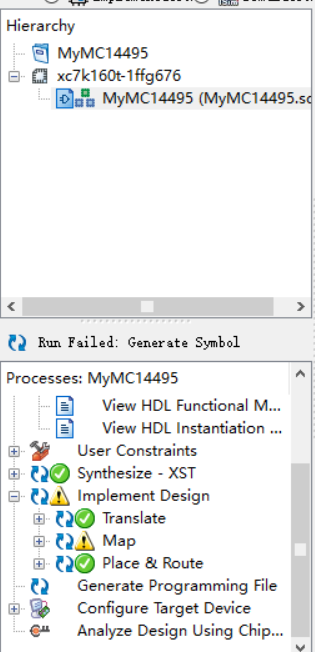
\includegraphics[width=0.3\textwidth]{3.png}
	\caption{\label{Lab6}检验}
	\end{figure}
完成Synthesize-XST,Implement Design,Manage Configuration Project(iMPACT)
最后Create Schematic Symbol,生成逻辑符号图供后序实验使用.

\subsubsection{对原理图进行仿真模拟}
导入仿真激励代码,并且生成波形图检验
\subsubsection*{仿真激励代码}
\begin{lstlisting}[language=verilog]
    `timescale 1ns / 1ps

    module MyMC14495_tb();
    
    // Inputs
      reg D0;
      reg D1;
      reg D2;
      reg D3;
      reg LE;
      reg point;
    
    // Output
      wire p;
      wire a;
      wire b;
      wire c;
      wire d;
      wire e;
      wire f;
      wire g;
    
    // Instantiate the UUT
      MyMC14495_HDL UUT (
      .D0(D0), 
      .D1(D1), 
      .D2(D2), 
      .D3(D3), 
      .LE(LE), 
      .point(point), 
      .p(p), 
      .a(a), 
      .b(b), 
      .c(c), 
      .d(d), 
      .e(e), 
      .f(f), 
      .g(g)
      );
    // Initialize Inputs
      integer i;
      initial begin
        //$dumpfile("MyMC14495_HDL.vcd");
        //$dumpvars(1, MyMC14495_HDL_tb);
    
        D3 = 0;
        D2 = 0;
        D1 = 0;
        D0 = 0;
        LE = 1'b0;
        point = 0;
        
        for (i=0; i<=15; i=i+1) begin
          {D3,D2,D1,D0}=i;
          point = i;
          #50;
        end
          
        #50;
        LE = 1'b1;
        #10;
      end
    endmodule
    
\end{lstlisting}
\subsubsection*{测试代码解释}
输入信号:\{D3,D2,D1,D0\},共同用于表示想要输出的数字(二进制形式)
LE是灯光使能信号,由于实验板是负逻辑,因此LE=0,可以显示数字, LE=1则不显示数字
point是控制小数点是否显示的信号,point=1时小数点显示

在测试模块中创建相应的变量:Input:D0,D1,D2,D3,LE,point.
Output:p,a~g.他们对应相应控制的七段数码管和小数点

创建测试的MyMC14496\_HDL模块,其名称为UUT,供后序的测试使用
在测试过程中通过循环对\{D3,D2,D1,D0\}的数值从0到15依次进行遍历,并且对point的值进行相应的修改,循环每次间隔50个单位时间
在循环结束后将LE设置为1,进行使能情况的判断



\subsection{用MyMC14495实现数码管显示}
\subsubsection{绘制DispNumber\_sch工程原理图}
导入前面产生的.sym和.vf文件,调用MyMC14495模块
    \begin{figure}[H]
	\centering
	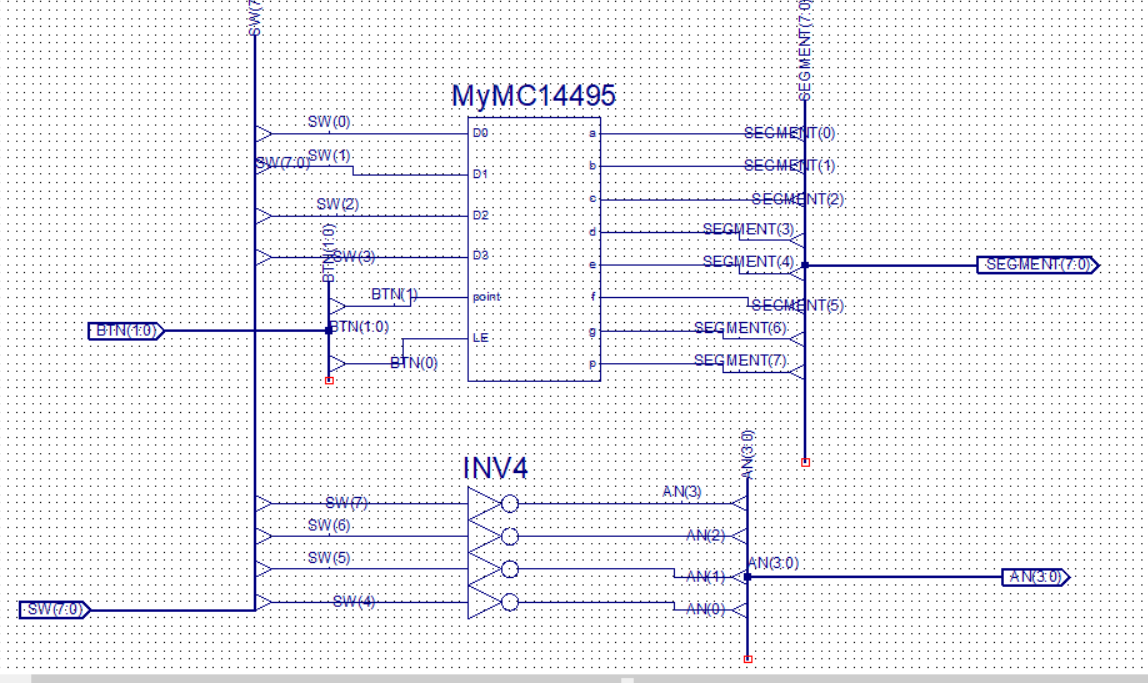
\includegraphics[width=0.6\textwidth]{4.png}
	\caption{\label{Lab6}原理图}
	\end{figure}

\subsubsection{下版验证}
导入引脚约束文件,将生成的.bit文件导入sword实验板进行下版验证

\section{实验结果与分析}

\subsection{原理图设计实现显示译码模块MyMC14495}
\subsection*{模拟仿真产生的波形图如下}
    \begin{figure}[H]
	\centering
	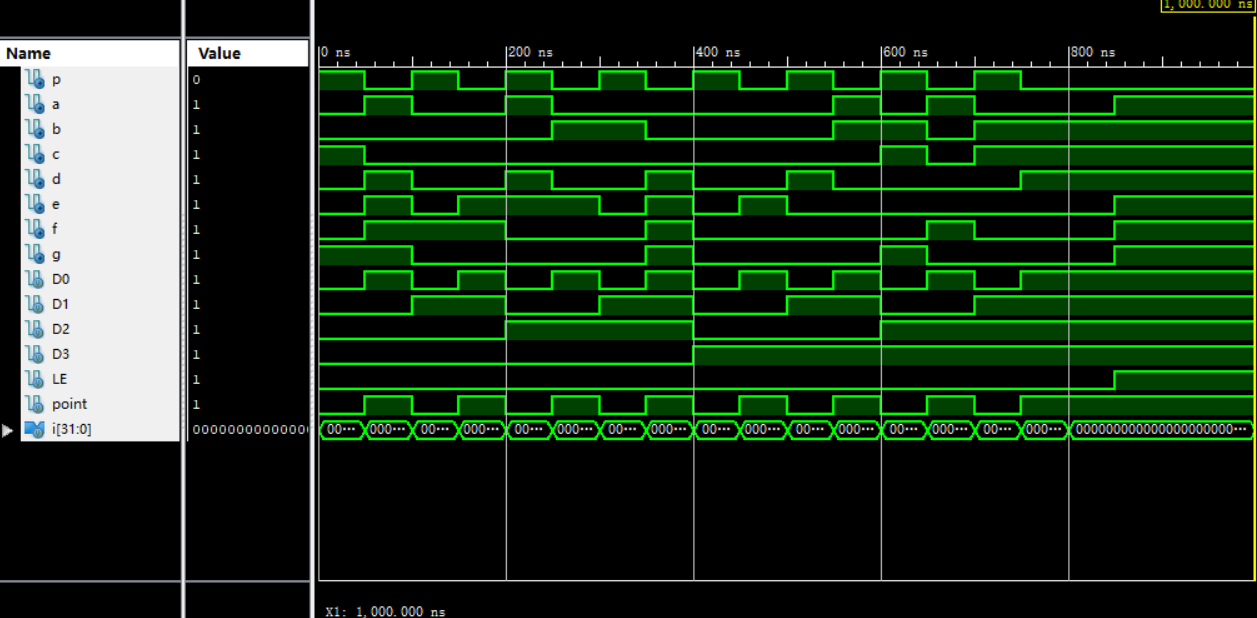
\includegraphics[width=0.7\textwidth]{2.png}
	\caption{\label{Lab6}波形图}
	\end{figure}

\subsection*{波形图分析}
输出p是输入信号取反得到的,可以看到,p的信号始终与point的信号保持相反
a~g的信号对应七段数码管的控制信号,输出的结果可以与真值表相对应
例如:当输入为\{0,1,0,0\},根据真值表,a,d,e,的值为1,其余信号的值为0,波形图上信号对应显示了相应的值
其他情况的输入也都与真值表所对应的吻合,可以验证所画的原理图是正确的
在波形图的后段,LE信号为1,因此信号a~g的输出均全为1.

\subsection{用MyMC14495实现数码管显示}
\subsection*{下版验证结果与分析:}
\subsection*{LE=1情况}
    \begin{figure}[H]
	\centering
	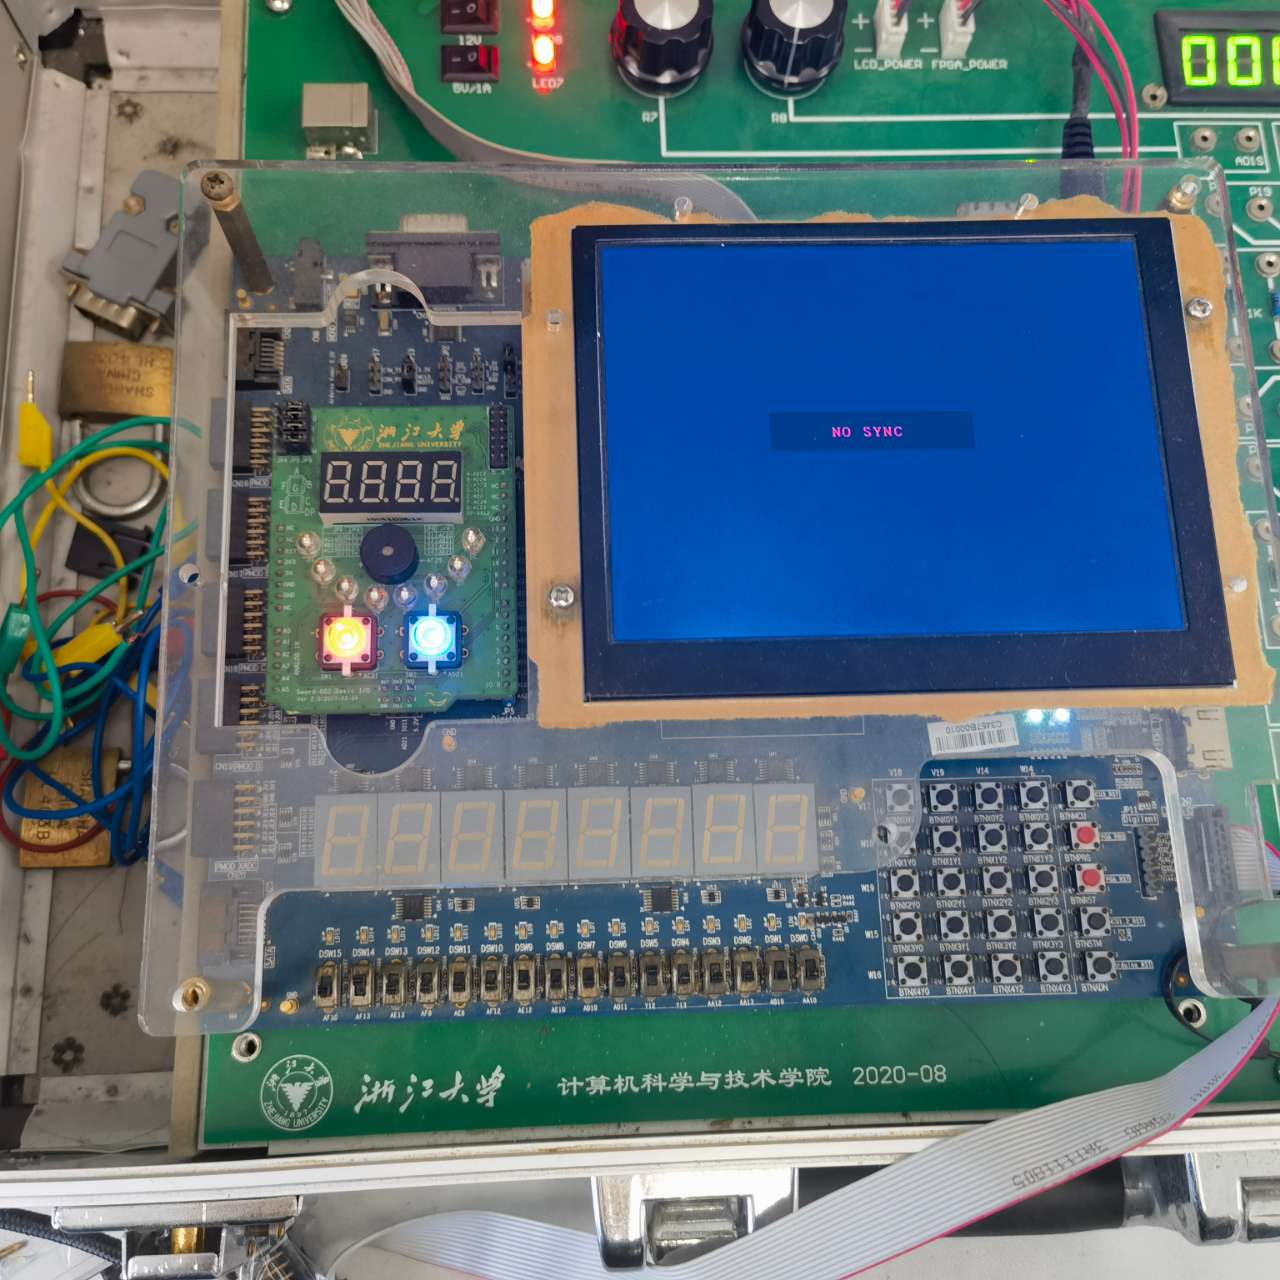
\includegraphics[width=0.5\textwidth]{5.jpg}
	\caption{\label{Lab6}下版验证}
	\end{figure}
\subsection*{分析:}
当拨动控制LE的开关时,使能情况为关闭,这时无论怎样改变开关的情况都没有灯闪亮

\subsection*{控制相应的数字产生:}
    \begin{figure}[H]
	\centering
	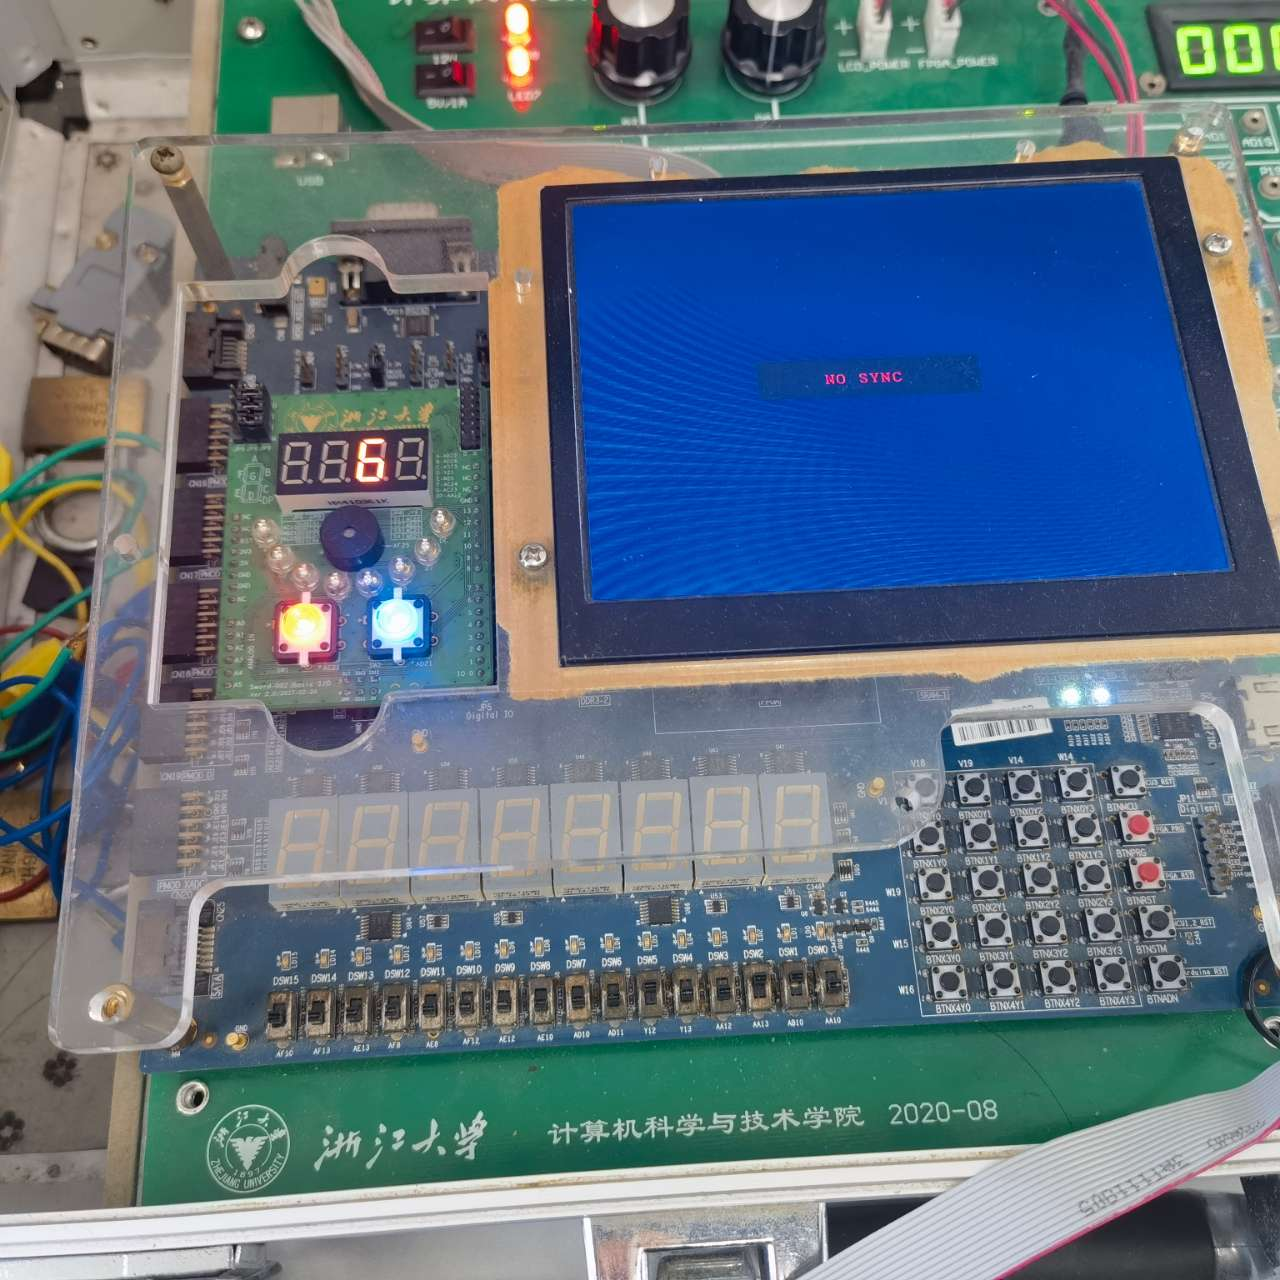
\includegraphics[width=0.4\textwidth]{6.jpg}
	\caption{\label{Lab6}下版验证}
	\end{figure}

    \begin{figure}[H]
    \centering
    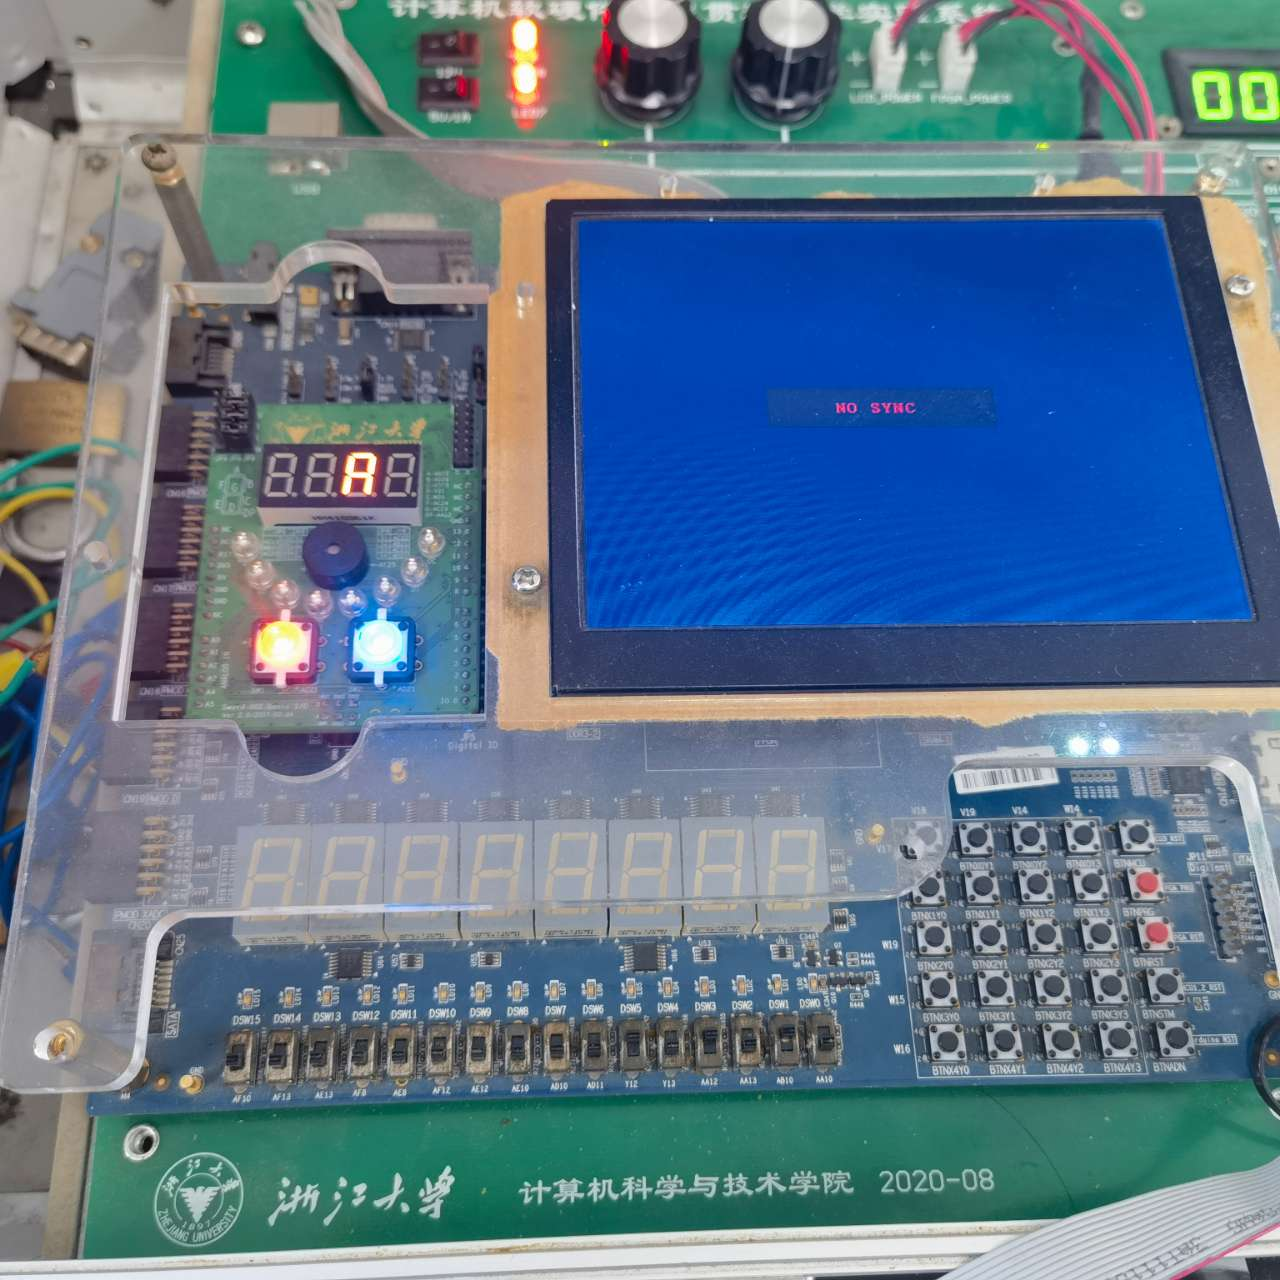
\includegraphics[width=0.4\textwidth]{7.jpg}
    \caption{\label{Lab6}下版验证}
    \end{figure}

    \begin{figure}[H]
    \centering
    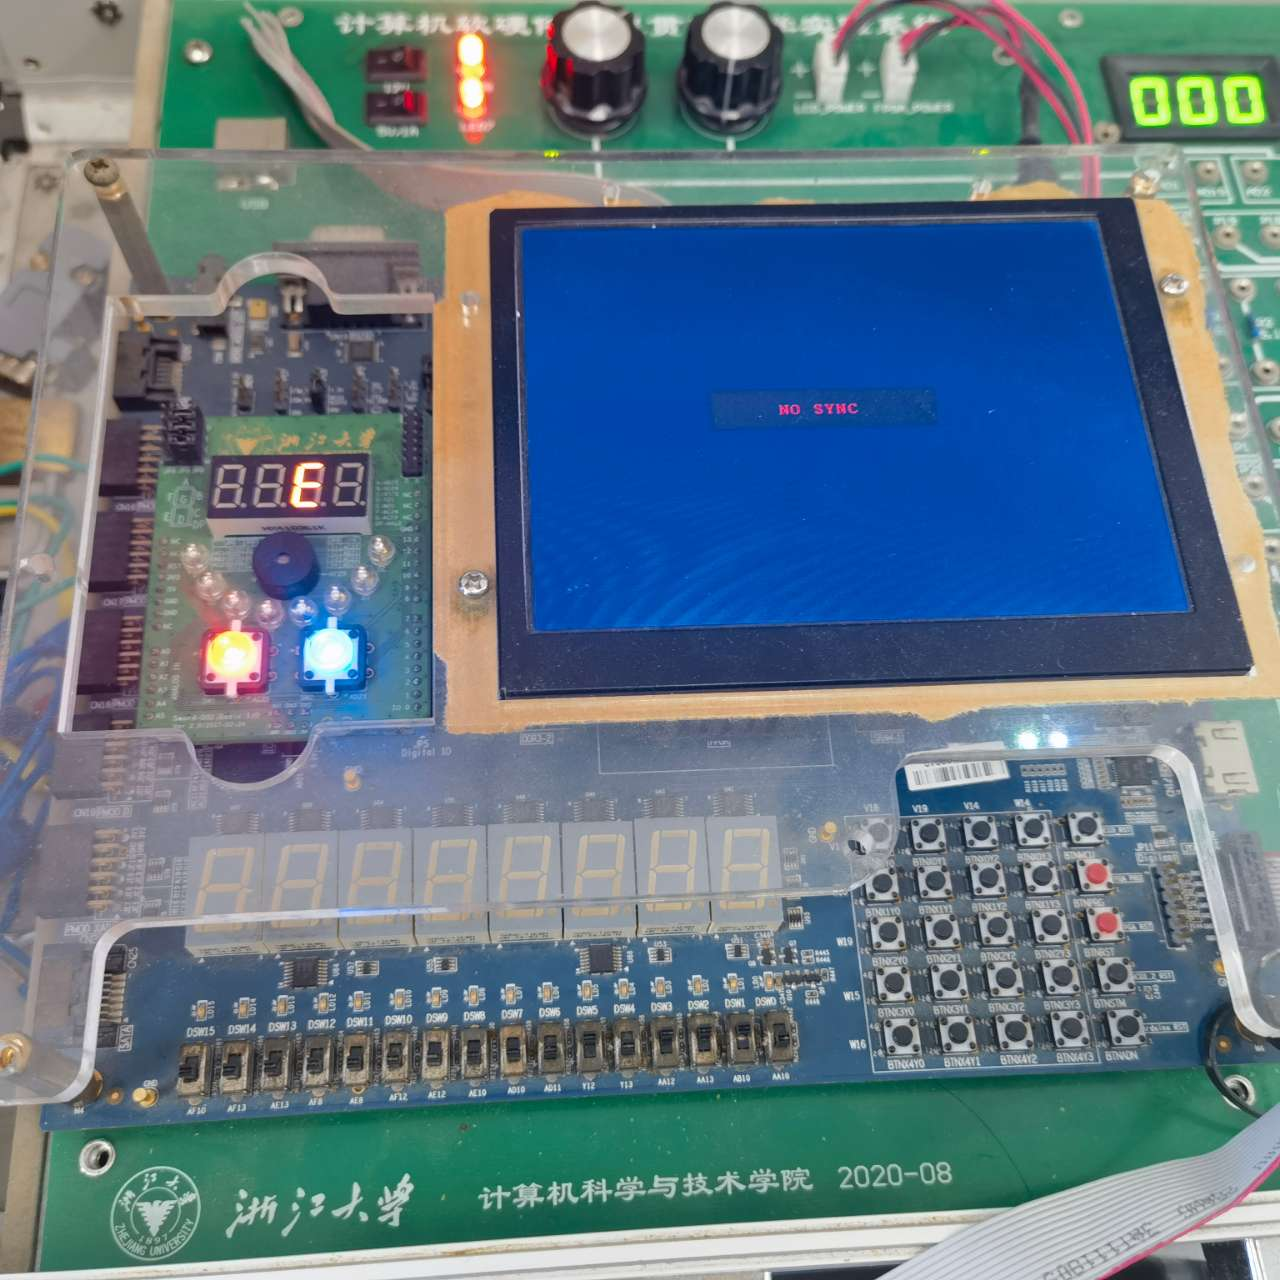
\includegraphics[width=0.4\textwidth]{8.jpg}
    \caption{\label{Lab6}下版验证}
    \end{figure}
\subsection*{分析:}
通过控制开关的拨动表示出对应的数字(二进制形式),在实验板上就会显示出相应的16进制数字
在这一部分实验中调用了MyMC14495模块进行使用,当在实验板上给定相应的输入时,输出所绑定的数码管会获得一个相应的输出,如果输出为0那么相应的数码管闪亮,反之则不闪亮
对应闪亮的数码管,根据实验原理的设置,他们之间的组合便显示出了相应的数字.

\subsection*{小数点控制}

    \begin{figure}[H]
    \centering
    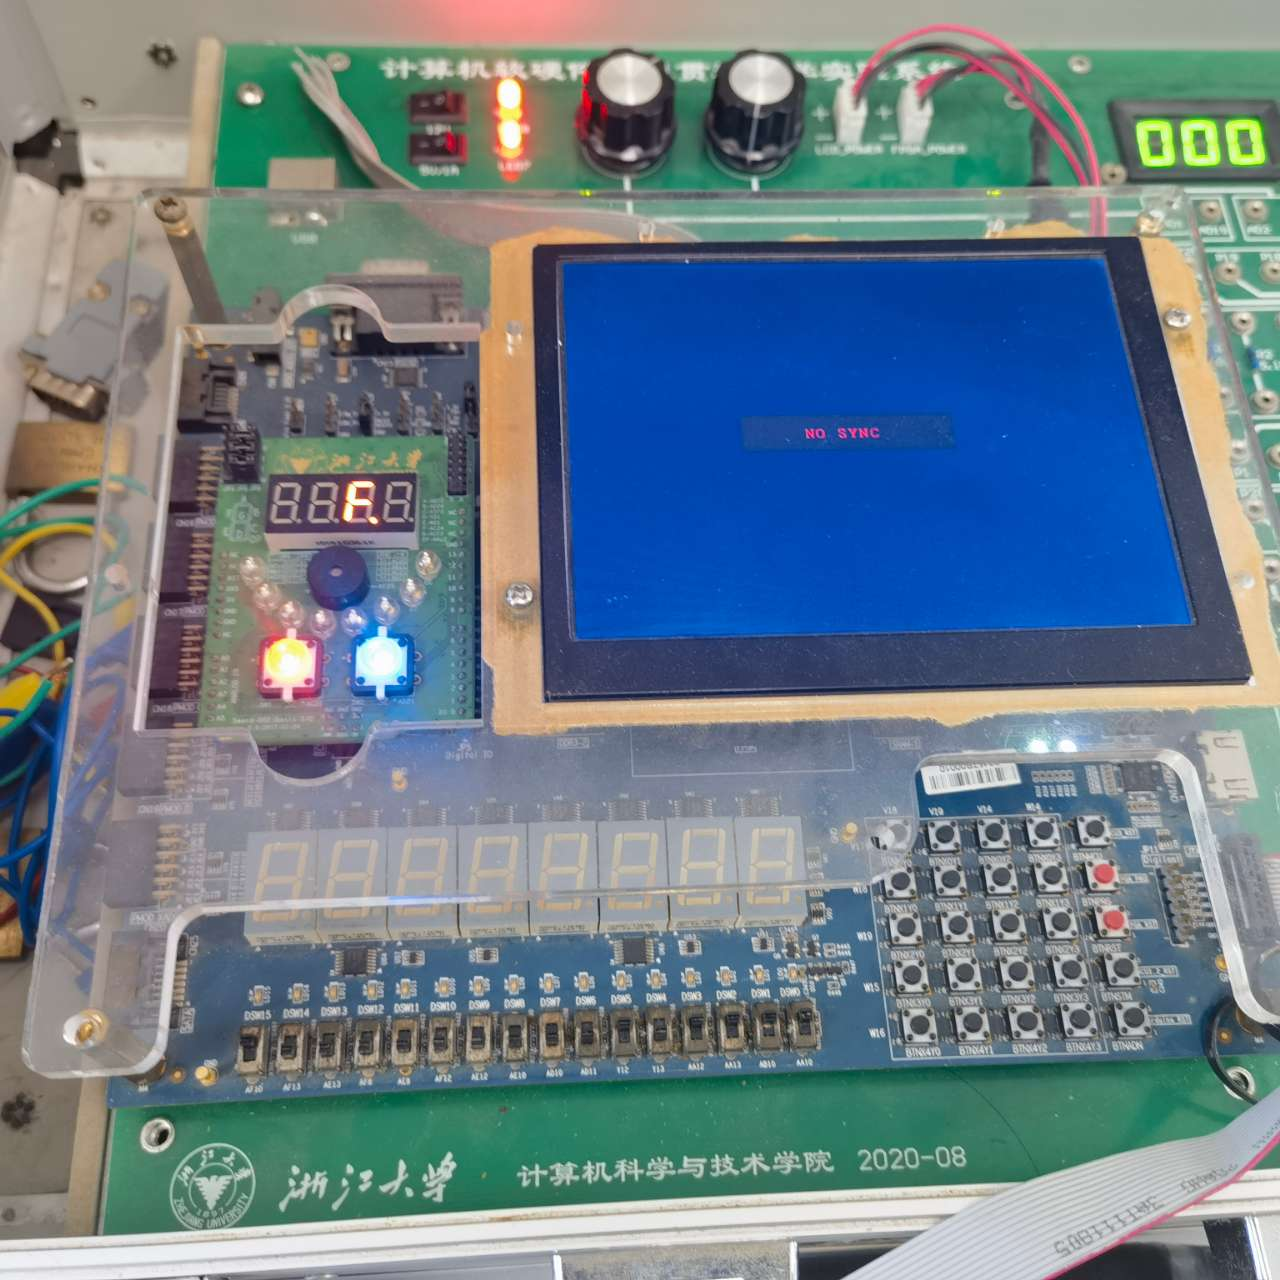
\includegraphics[width=0.4\textwidth]{10.jpg}
    \caption{\label{Lab6}下版验证}
    \end{figure}
\subsection*{分析:}
当控制小数点的部分的开关被拨动时,可以看到,数码管处显示了一个点.


\section{讨论与心得}
本次实验遇到的问题是:(1)由于实验的原理图过于复杂,画原理图时耗费了很长的时间,开始由于不会调节画布的大小,
导致根本画不下所有的电路,改变画布大小后才继续画出; (2)在画完原理图进行波形的验证时发现,有一个信号对应的
输出与真值表并不相符,但由于对线路进行了重新命名,因此很快找出了所存在的问题,问题得以解决; (3)在重新绘制原理
图后,再次生成新的.vm文件时无法重新生成,在将错误的.vm文件删除后问题才得以解决.

\section{Bonous}
\section*{完成MyMC15595\_HDL.v}
\begin{lstlisting}[language=verilog]
    `timescale 1ns/1ps

    module MyMC14495_HDL(
      input D0, D1, D2, D3,
      input LE,
      input point,
      output reg p,
      output reg a, b, c, d, e, f, g
    );
    
      `define MC14495_NUM {D3, D2, D1, D0}
      `define MC14495_OUT {a, b, c, d, e, f, g}
    
      always@(*) begin
        if(1'b0 == LE) begin
          /* Able to print */
          // Point
          p = !point;                             // fill sth in ()
          // Num(0~9, A~F)
          case(`MC14495_NUM)
            4'h0: `MC14495_OUT = 7'b000_0001;
            /* Complete the following code. */
            4'h1: `MC14495_OUT = 7'b100_1111;
            4'h2: `MC14495_OUT = 7'b001_0010;
            4'h3: `MC14495_OUT = 7'b000_0110;
            4'h4: `MC14495_OUT = 7'b100_1100;
            4'h5: `MC14495_OUT = 7'b010_0100;
            4'h6: `MC14495_OUT = 7'b010_0000;
            4'h7: `MC14495_OUT = 7'b000_1111;
            4'h8: `MC14495_OUT = 7'b000_0000;
            4'h9: `MC14495_OUT = 7'b000_0100;
            4'hA: `MC14495_OUT = 7'b000_1000;
            4'hB: `MC14495_OUT = 7'b110_0000;
            4'hC: `MC14495_OUT = 7'b011_0001;
            4'hD: `MC14495_OUT = 7'b100_0010;
            4'hE: `MC14495_OUT = 7'b011_0000;
            4'hF: `MC14495_OUT = 7'b011_1000;
            /* end of your code */
            default: `MC14495_OUT = 7'bxxx_xxxx;
          endcase
    
        end else begin
          // Print nothing (LE == 1)
          `MC14495_OUT = 7'b111_1111;                  // fill sth in ()
          p = !point;                             // fill sth in ()
        end
    
      end
    
    endmodule
\end{lstlisting}
\section*{代码解释:}
在case语句中,将输入对应的数字所得到的真值表的值对相应的结果进行匹配写入即可
p的输出值时输入信号point的取反
当LE=1对应数码管的输出均为1

\section*{波形图分析:}
    \begin{figure}[H]
    \centering
    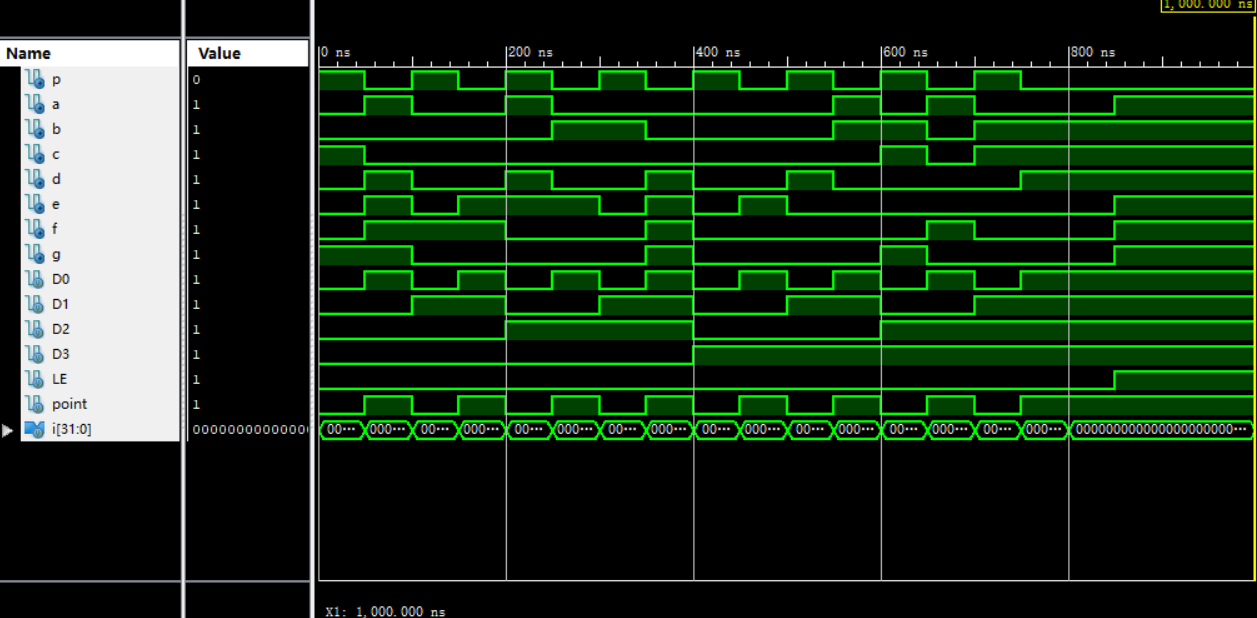
\includegraphics[width=0.6\textwidth]{2.png}
    \caption{\label{Lab6}波形图}
    \end{figure}
\section*{分析:}
此波形图对应的结果和通过原理图得到的波形图的结果是一致,可以验证程序的正确性.

\end{document}